\subsection{Code Smells}
\label{smells:results}
Using the sampling approach described in section~\ref{sampling}, we sampled 25 best practices in javascript from AirBNB javascript coding style guide~\cite{airbnb_code}. 
We then compared Copilot suggestions when prompted with an input(shown in section~\ref{input}) to trigger a code suggestion from Copilot and present our results using evaluation approach~(shown in section~\ref{evaluation}).

Copilot suggested the best practice from the AirBNB javascript coding style guide~\cite{airbnb_code} for 3 out of the 25 coding standards we tested, i.e, 3 out of 25 instances Copilot had the recommended best practice as its top suggestion.
Moreover, only 5 out of remaining 22 coding scenarios had the best practice in Copilot top 10 suggestions currently viewable. 
Copilot did not have the best practice in any of its top 10 suggestions for 17 scenarios out of 25 coding scenarios we tested.

The results show that Copilot did not suggest the recommended best practice as its first suggestion in the majority (88\%) of the best practices we tested.
As Copilot is closed source, we cannot find the reason behind this but one could argue that lack of data for JavaScript compared to python could be a reason for this behaviour. 

The results show that Copilot performed worse than the language idioms~(shown in chapter~\ref{idioms}).  This shows that current AI-supported
code completion tools like Copilot is not yet capable of suggesting the best practices in its suggestions even though the best practices are the sampled from widely accepted coding style guide.

There could be many reasons for this performance like the public repositories do not always follow coding standards, Copilot cannot detect coding style from repositories that have contribution guides including the coding standards followed in the project. 
Copilot being closed source we cannot investigate the potential reasons behind this behavior and recommend ways to fix this issue improving the performance of Copilot.

We did not test Copilot for suggesting project specific coding styles because Copilot does not have the feature to customise its suggestions based on preferences~\cite{Copilot-web}.
However, \cct{} like Copilot should follow coding style guides and adapt their code suggestions to match the coding style used in the project. 
For example, if a user is working on a project where one of the coding style guideline says to leave a blank line after blocks and before the next statement~\cite{airbnb_code}. As a productivity tool, the ideal behaviour for \cct{} like Copilot is to detect the coding style guideline from existing code or a coding style document in the project and always suggest code that follows the guidelines.

Figure~\ref{fig:bp_1} shows the Best Practice for Copying Array Contents, showing user input (i.e., Human Input), the top suggestion by Copilot and the recommended way suggested by AirBNB JavaScript coding style guide~\cite{airbnb_code}.

\begin{figure}[hbt!]
    \centering
    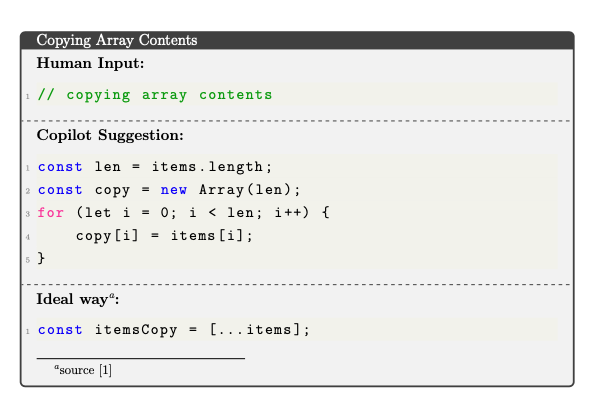
\includegraphics[width=\linewidth]{Figures/bp_1.png}
    \caption{Best Practice for Copying Array Contents and Copilot Suggestion.}
    \label{fig:bp_1}
\end{figure}

\cct{} like Copilot should learn to suggest best practices to avoid code smells, detect coding style of the project and adapt its coding suggestions in order to be helpful for a user as a productivity tool. 

% \begin{tcolorbox}[title=Copying Array Contents,boxsep=.15mm]
%     %https://tex.stackexchange.com/questions/337909/tcolorbox-tcbline-style
% \textbf{Human Input:}
% \begin{lstlisting}[language=JavaScript]
% // copying array contents
% \end{lstlisting}
% \tcbline
% \textbf{Copilot Suggestion:}
% \begin{lstlisting}[language=JavaScript]
% const len = items.length;
% const copy = new Array(len);
% for (let i = 0; i < len; i++) {
% 	  copy[i] = items[i];
% }
% \end{lstlisting}
% \tcbline
% \textbf{Ideal way\footnote{source \cite{airbnb_code}}:}
% \begin{lstlisting}[language=JavaScript]
% const itemsCopy = [...items];
% \end{lstlisting}
% \end{tcolorbox}

%%%%%% TODO: remember to update the screenshot if the source citation is different from the citation in the text %%%%%%

Table~\ref{tab:all_bp} shows the complete list of all the best practices we tested on Copilot sampled from the AirBNB Coding Style guide~\cite{airbnb_code} and the ranking of the best practice in Copilot suggestions (if it exists).
All the best practices shown in Table~\ref{tab:all_bp} can be found in the \repl{} including the code used as input (i.e., human input), the top suggestion by Copilot and the best practice from AirBNB JavaScript coding style guide~\cite{airbnb_code}.

\begin{table}[hbt!]
        \centering
    \begin{tabular}{|c|c|c|}
        \hline

        \textbf{S No.} & \textbf{Best Practice  Title} & \textbf{Copilot Suggestion Matched?} \\
         & & (out of 10 suggestions) \\
         \hline
         1 & Usage of Object method shorthand & No \\
         \hline
         2 & Array Creating Constructor & 6\textsuperscript{th} \\
         \hline
         3 & Copying Array Contents  & No \\
         \hline
         4 & Logging a Function &  No \\
         \hline
         5 & Exporting a Function & No \\
         \hline
         6 & Sum of Numbers & 9\textsuperscript{th} \\
         \hline
         7 & Accessing Properties & 1\textsuperscript{th} \\
         \hline
         8 & Switch case usage & No \\
         \hline
         9 & Return value after condition & No \\
         \hline
         10 & Converting Array-like objects  & No \\
         \hline
         11 & Create two references & 5\textsuperscript{th} \\
         \hline
         12 & Create and reassign reference & No \\
         \hline
         13 & Shallow-copy objects  & No \\
         \hline
         14 & Convert iterable object to an array & No \\
         \hline
         15 & Converting array like object to array & 1\textsuperscript{st} \\
         \hline
          16 & Multiple return values in a function & No \\
          \hline
          17 & Return string and variable name & No \\
          \hline
          18 & Initialize object property & No \\
          \hline
          19 & Initialize array callback & No \\
          \hline
          20 & Import module from file & 6\textsuperscript{th} \\
          \hline
          21 & Exponential value of a number & No \\
          \hline
          22 & Increment a number & 2\textsuperscript{nd} \\
          \hline
          23 & Check boolean value & 1\textsuperscript{st} \\
          \hline
          24 & Type casting constant to a string & No \\
          \hline
          25 & Get and set functions in a class & No \\
          \hline
    \end{tabular}
    \caption{List of all JavaScript best practices tested on Copilot.}
    \label{tab:all_bp}
\end{table}
